\documentclass[a6paper, 10pt, twoside]{article}
%\usepackage[T1]{fontenc}
\usepackage[british]{babel}
\usepackage[utf8]{inputenc}
\usepackage{float, graphicx,amsmath,amsfonts,cite,enumerate,tabularx}
\usepackage[final]{pdfpages}
\usepackage{wrapfig}
\usepackage[margin=0.3in]{geometry}
\usepackage{sidspaltHack}
\usepackage{digital}

%\usepackage[framed,numbered,autolinebreaks,useliterate]{mcode}
\newcommand{\notis}[1]{\begin{flushright}\textit{#1}\end{flushright}}

\setlength{\oddsidemargin}{-0.37in}
\setlength{\evensidemargin}{-0.47in}
\setlength{\textwidth}{215pt}

\pagestyle{empty}

\begin{document}
\nysida{4}{}
\noindent
\chaptertitlenobr{$\Delta\delta$}{Visor till destillat}
\vspace{10pt} \\
\Large Supregler\\ % Om du ändrar i denna text, ändra även motsvarande i /parser/inject/04/
\small 
Varje människa som vill föra en regelmässig diet i mat och dryck tager sig följande styrketårar.

Förutsatt att en icke svultit eller törstat dagen innan besväras en dagligen av slem i halsen eller så kallade tuppar, varför en börja efter uppvaknandet med tuppsupen. Den kan tagas på sängen. En stund därefter och sedan en tagit en liten motion följer den uppfriskande bäsken. Vidare en klar för att borttaga bäskens eftersmak. Nu dricker en sitt kaffe varefter kaffesupen ej förgätes. Vid frukosten tages aptitsupen, fisksupen och halvan.

Nu inträder arbetstiden varunder blott fyllehundar supa. När middagen är serverad tages aptitsupen och innan en skiljer sig från middagsbordet, klacken. Därefter under måltiden supen på fisken, halvan och tersen. På eftermiddagen sedan en tagit sin middagstupplur drickes kaffe varefter kaffesupen ej försummas. Den som ej dricker kaffe är berättigad att istället för kaffe taga sig en klar. Därefter följa sexan som näst efter aptitsupen är den angelägnaste.

Nu ha vi tedags, men en sann patriot dricker inte denna dryck, som gör magen kvalmig, utan då en sätter sig till spelbordet, tar en sig istället en spelsup, därefter drickes toddy och mellan varje sådan är en berättigad till mellanbindare och äro glasen ej allt för stora drickes tre toddar och följdaktligen tages också två mellanbindare. Vid kvällsmåltiden de tre ordinarie måltidssuparna och då en stiger i sängen bör en ej glömma loppsupen och härmed är dagen till ända. 

\newpage
Dessa 21 supar och 3 toddar äro en måttlig kropps dagliga diet. Likväl kan den vid träget och tröttande arbete förstärkas. En uppfriskar sig då med styrkesupen. Vad därutöver är kan möjligen urarta till rummel och bör därför undvikas. I ovanstående äro emellertid ej inberäknade kyrksupen, tankeställaren, handelssupen och släpsupen.
\vspace{-5pt}
\notis{Utdrag ur en pastors anteckningar, 1809.}
\vspace{-15pt}
\begin{center}
\Large{De sjutton suparnas intagande}
\end{center}
\vspace{-15pt}
\begin{table}[!h]
\begin{tabularx}{0.85\textwidth}{l l}
\small 1. Helan&\small Intages skyndsamt. AHH! \\
\small 2. Halvan&\small Intages frejdligt.\\
\small 3. Tersen&\small Intages glatt.\\
\small 4. Kvarten&\small Intages gärna.\\
\small 5. Kvinten&\small Intages hellre.\\
\small 6. Rivan&\small Intages också\\
\small 7. Septen&\small Intages av bara farten.\\
\small 8. Rafflan&\small Halkar ner.\\
\small 9. Rännan&\small Gär väl an!\\
\small 10. Smuttan&\small NÅJA!\\
\small 11. Smuttans ungar&\small Det gick ju igår.\\
\small 12. Femton droppar&\small Det skall gå!\\
\small 13. Lilla Manasse&\small Intages flängande.\\
\small 14. Lilla Manasses bror&\small Intages krängande.\\
\small 15. Kreaturens uppståndelse&\small Intages hängande.\\
\small 16. Absolut sista supen&\small Intages knästående.\\
\small 17. Den bleka dödens dryck&\small Sköljes ned med pilsner.
\end{tabularx}
\end{table}
\vspace{-15pt}
\begin{table}[!h]
  \begin{tabular}{|r|}
\hline
\textit{"It's good for two things: degreasing}\\ \textit{engines and killing brain cells."}\\\textit{- Cypher, "The Matrix" (1999)} \\
\hline
  \end{tabular}\
\end{table}

% TODO: Move to below chapter title
\small

\nysida{4}{1}
\noindent
\begin{center}
    \songtitle{$\delta1$a}{Helan går}
\end{center}
\begin{lyrics}
Helan går, \\
sjung hopp faderallan lallan lej! \\
Helan går, \\
sjung hopp faderallan lej! 
\vspace{5pt} \\
Och den som inte helan tar, \\
hen heller inte halvan får. \\
Helan går (\textit{supen intages})\\
Sjung hopp faderallan lej! 
\end{lyrics}
\begin{center}
    \songtitle{$\delta1$b}{Hell and gore} 
    \mel{Helan går}
\end{center}
\begin{lyrics}
Hell and Gore, \\
Chung Hop father Allan, Allan ley! \\
Hell and Gore, \\
Chung Hop father Allan ley!
\vspace{5pt} \\
On handsome in the hell and tar \\
Hell are in the half and four \\
Hell and Gore! \\
Chung Hop father Allan ley! 
\end{lyrics}
\begin{center}
    \songtitle{$\delta1$c}{Et langue d'or} 
    \mel{Helan går}
\end{center}
\begin{lyrics}
Et langue d'or, joue haute fadeur a l'an la langue laide! \\
Et langue d'or, joue haute fadeur a l'an laide! \\
Octane somme mine te et loitain, \\
A ni te et leur halle vend fort. \\
Et langue d'or! \\
Joue haute fadeur a l'an laide! 
\end{lyrics}

\newpage
\noindent
\begin{center}
    \songtitle{$\delta1$d}{Imbelupet} 
    \mel{Kors på Idas grav}
\end{center}
\begin{lyrics}
\small Imbelupet glaset står på bräcklig fot. \\
Svala pilsnerpavor luta sig därmot. \\
Men därnere, miserere... 
\vspace{5pt} \\
...uti magens mörka djup \\
sitter Djävulen och väntar på en sup. 
\vspace{5pt} \\
...uti magens dunkla valv \\
sitter Djävulen och ropar på en halv. 
\vspace{5pt} \\
...uti magen kors och tvärs \\
irrar Djävulen och skriker på en ters. 
\vspace{5pt} \\
...uti magens tom och svart \\
sitter Djävulen och skränar på en kvart. 
\vspace{5pt} \\
...uti magens labyrint \\
sitter Djävulen och tjoar på en kvint. 
\vspace{5pt} \\
...uti magens slingerväxt \\
sitter Djävulen och skriar på en sext. 
\vspace{5pt} \\
...uti magen heluppknäppt \\
sitter djävulen och vrålar på en sept. 
\vspace{5pt} \\
...uti magen varm och kvav \\
sitter djävulen och väser på oktav. 
\end{lyrics}

\newpage
\noindent
\begin{center}
    \songtitle{$\delta1$e}{Vem sade ordet "skål"?} 
    \mel{Vårvindar friska}
\end{center}
\begin{lyrics}
Vem sade ordet "skål" här vid bordet,\\
viskande for det sällskapet kring.\\
Fattom kristallen, nubben är kall den,\\
stiger åt skallen, pling, plang, pling.\\
Käraste vänner välkomna hit\\
känn hur det bränner god akvavit.\\
Nu lilla hutten går i kaputten\\
skål lilla tutten, pling, plang, pling.
\end{lyrics}
\begin{center}
    \songtitle{$\delta1$f}{Ubåten} 
    \mel{Jazzgossen}
\end{center}
\begin{lyrics}
Å så kommer det en ångbåt, \\
och den säger: "Tut-tut-tut!" \\
Å så kommer det en ubåt, \\
och den säger: \\
\textit{(Gurgla nubben) }
\end{lyrics}

\begin{center}
    \Large $\delta1$g. Heltal rho\\ 
    \mel{Helan går}
\end{center}
\begin{lyrics}
$\mathbb{Z}$ $\rho$\\ 
7 8 $\forall$ $\lambda$ $\pi$\\ 
$\mathbb{Z}$ $\rho$\\ 
7 8 $\forall$ $\lambda$ $\pi$\\ 
$\text{\^{}}$ $\otimes$ $\int$\\
n $\vee$ $\neg$ $\lfloor$ $\nabla$ $\rfloor$\\
$\mathbb{Z}$ $\rho$ ($\forall$ droppar $\in$ glaset, sup)\\
7 8 $\forall$ $\pi$!
\end{lyrics}
\auth{Leo Tikkanen, F-20}

\nysida{4}{2}
\noindent
\begin{center}
    \songtitle{$\delta2$a}{När helan en tagit} 
    \mel{Skånska slott och härresäten}
\end{center}
\begin{lyrics}
När helan en tagit \\
och halvan ska dricka, \\
Det är som att kyssa \\
en nymornad kära. 
\vspace{5pt} \\
Ju mera en får, \\
desto mer vill en ha, \\
En ensammer jävel \\
gör alls ingen gla'. 
\end{lyrics}
\vspace{60pt}
\begin{center}
    \songtitle{$\delta2$b}{Halvan} 
    \mel{Pojkarne}
    \sheetmusicnoticenormal{Noter finns i notkapitlet}
\end{center}
\begin{lyrics}
Hur länge skall på borden\\ 
den lilla halvan stå? \\
Skall snart ej höras orden: \\
Nu halvan går, låt gå!
\vspace{5pt} \\
Det ärvda vikingsinne \\
till supen trår igen, \\
och helans trogna minne \\
i halvan går igen.
\end{lyrics}

\newpage
\noindent
\begin{center}
    \songtitle{$\delta2$c}{Angorakatten} 
    \mel{Vi går över daggstänkta berg}
\end{center}
\begin{lyrics}
Det var en gång en vanlig bonnakatt, fallera, \\
som älskade en hel-angorakatt, fallera! \\
Och följden blev en jamare, \\
men den blev mycket tamare, \\
för den var blott en halv-an-gor-akatt, fallera. 
\end{lyrics}
\begin{center}
    \songtitle{$\delta2$d}{Helan gick} 
    \mel{Amanda Lundbom}
\end{center}
\begin{lyrics}
Helan gick i vänstra foten, \\
bom-faderia, faderareralla. \\
Gudskelov, så vet jag boten, \\
bom-faderi, faderallanlej! \\
Halvan ställer saken rätt, \\
bom-faderi, faderallanlej \\
Hugg i! \\
På nubbar blir en aldrig mätt, \\
bom-faderi, faderallanlej! 
\end{lyrics}
\begin{center}
    \songtitle{$\delta2$e}{Helan rasat} 
    \mel{Längtan till landet}
\end{center}
\begin{lyrics}
Helan rasat ned i våra magar, \\
sQuvValpar nu på botten mol allen. \\
I sin ensamhet den bittert klaga: \\
"Det är svårt att bara vara en." \\
Snart är halvan här, den härliga supen, \\
alkoholiskt ren och silverklar, \\
Dansar som en vårbäck ned genom strupen \\
Hamnar --- plask! --- i helans budoir. 
\end{lyrics}

\nysida{4}{3}
\noindent
\begin{center}
    \songtitle{$\delta3$a}{Nubbekantat} 
    \mel{Smedsvisa}
\end{center}
\begin{lyrics}
Att höja en skål kan nog vara rätt \\
men måttfullhet krävs för att ej halka snett. \\
Av drycker är tersen särklassigt bäst \\
som tömmes av vänner på fest. \\\digitalonly{\\}
Så, blott några koppar är allt vi vill ha \\
och bäska droppar måste det va'. \\
Men vägen till tersen är ganska lång \\
så helan vi tar med en gång. 
\vspace{5pt} \\
Nu har vi väl sagt varandra gutår, \\
lagt bort våra titlar så gott som det går, \\
inlett med vår bordsvän konversation, \\
då strupen vill ha solution. \\\digitalonly{\\}
Så, blott några koppar är allt vi vill ha \\
och bäska droppar måste det va'. \\
Ty talet gör halsen otroligt torr \\
så halvan vi tar med en knorr. 
\vspace{5pt} \\
Om vi mot förmodan äter nån mat \\
så bytes vårt lammkött mot pizza på fat. \\
Den vådliga rätten får nog stå kvar \\
istället vi tar oss en klar. \\\digitalonly{\\}
Så, blott några koppar är allt vi vill ha \\
och bäska droppar måste det va'. \\
Av maten så blir en tjocker och fet \\
så tersen får bli vår diet. 
\end{lyrics}
\auth{Ur det 46:e Bergsspexet KrigEtt}

\newpage
\noindent
\begin{center}
    \songtitle{$\delta3$b}{Var Osquristina} 
    \mel{Te deum (Eurovision-signaturen)}
\end{center}
\begin{lyrics}
Var Osquristina som går på vår sektion \\
av äldre kollegor lärt en tradition, \\
att noga se om sin kondition, \\
Och högra armen ge motion. 
\end{lyrics}
\begin{figure}[!h]
\centering
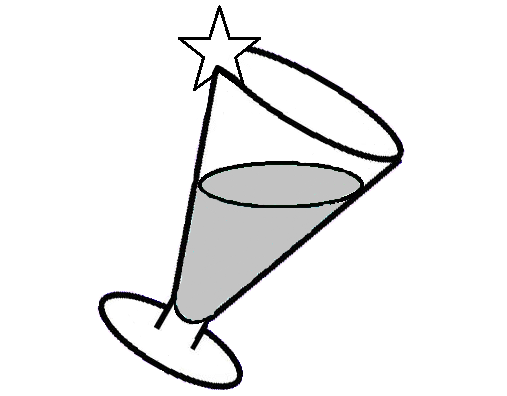
\includegraphics[width=0.5\textwidth]{nubbe.png}
\end{figure}
\begin{center}
    \songtitle{$\delta3$c}{Små nubbarna} 
    \mel{Små grodorna}
\end{center}
\begin{lyrics}
Små nubbarna, små nubbarna \\
är äckliga att se, \\
små nubbarna, små nubbarna \\
är äckliga att se.
\vspace{5pt}\\
Nu tar vi dom, nu tar vi dom, \\
så slipper vi dom se, \\
nu tar vi dom, nu tar vi dom, \\
så slipper vi dom se.
\end{lyrics}

\nysida{4}{4}
\noindent
\begin{center}
    \songtitle{$\delta4$a}{Planksaft}
    \songsubtitlelarge{(Längtan till baren)}
    \mel{Längtan till landet}
\end{center}
\begin{lyrics}
Törsten rasar uti våra strupar, \\
tungan hänger torr och styv och stel. \\
Men snart vankas stora långa supar, \\
var och en får sin beskärda del. \\
Snapsen kommer, den vi vilja tömma, \\
denna nektar lik Olympens saft \\
kommer oss att våra sorger glömma. \\
Snapsen skänker hälsa, liv och kraft. 
\vspace{5pt}\\
Fordom odlade en vindruvsrankor \\
av vars saft en bryggde ädelt vin. \\
Nu en pressar saften ur en planka, \\
doftande av äkta terpentin. \\
Höj nu bägaren o broder, syster, \\
låt den svenska skogen rinna kall, \\
genom strupen och om du är dyster, \\
låt oss dricka upp en liten tall. 
\vspace{5pt}\\
Helan tänder helig eld i själen, \\
halvan rosar livet som en sky, \\
tersen känns från hjässan ned i hälen, \\
kvarten gör en som en männska ny. \\
Låt oss skåla med varandra go' vänner \\
skål för vår levnads glada hopp. \\
Törstens eld på nytt i strupen bränner. \\
Leve livet skål och botten opp! 
\end{lyrics}

\newpage
\noindent
\begin{center}
    \songtitle{$\delta4$b}{Brännvin hit} 
    \mel{Skära havre}
\end{center}
\begin{lyrics}
Brännvin hit \\
och brännvin dit \\
och brännvin är det bästa. \\
Och fan den \\
som brännvin har \\
och inte bju'r sin nästa. 
\end{lyrics}
\vspace{10pt}
\begin{center}
    \songtitle{$\delta4$c}{Gums visa} 
    \mel{Skära havre}
\end{center}
\begin{lyrics}
\vspace{-5pt}
Skål, kamrater, \\
livet är glatt, \\
och snart förgäta vi sorgen, \\
Vi söpo igår, \\
vi supa idag \\
och tar en sjujäkel i morgon!
\end{lyrics}

\nysida{4}{5}
\noindent
\begin{center}
    \songtitle{$\delta5$a}{Fkåne faft} 
    \mel{Helan går}
\end{center}
\begin{lyrics}
Fkåne faft, \\
En fydfvenfk faft med fällfam kraft. \\
Fkåne faft, \\
Den bäfta faft vi haft. 
\vspace{5pt}\\
Enf livfluft löfef, fläppef loff, \\
När fådan faft ferveraf off, \\
Fmakenf faft \\
Till landf, till luftf, till havf. 
\end{lyrics}
\begin{center}
    \songtitle{$\delta5$b}{Mera Skåne} 
    \mel{Internationalen}
\end{center}
\begin{lyrics}
Nu är det dags att taga supen; \\
den stärker varje svag fysik. \\
Den rinner ner igenom strupen, \\
river gott som en tolvtumsspik. 
\vspace{5pt}\\
Den är vårt hopp mot gula faran, \\
vår tröst vid varje bleklagd sorg. \\
Den stärker oss mot mask i magen, \\
starkare än Svea borg! 
\vspace{5pt}\\
Mera Skåne i glasen, \\
flera glas på vårt bord! \\
Mera bord på kalasen, \\
fler kalas på vår jord! \\
Mera jordar kring månen, \\
flera månar kring Mars! \\
Mera marscher till Skåne! \\
Mer Skåne gubevars, bevars, bevars! 
\end{lyrics}

\newpage
\noindent
\begin{center}
    \songtitle{$\delta5$c}{En cyklar för lite} 
    \mel{Väda vadmal}
\end{center}
\vspace{-5pt}
\begin{lyrics}
En cyklar för lite'. \\
En röker för mycke' \\
\textbf{och en är fasen så liberal  \\
när det det gäller maten och spriten. \\
En borde slutat för länge sedan\\
men denna sup är för liten.} \\
Vad tjänar att hyckla. \\
Tids nog får en cykla.
\vspace{5pt}\\
En badar för lite'. \\
En röker för mycke' \\
\textbf{och en är...}\\
Det kan inte skada. \\
Tids nog får en bada.
\vspace{5pt}\\
 En sover för lite'. \\
en röker för mycke' \\
\textbf{och en är...}\\
Njut var gudagåva! \\
Tids nog får en sova.\\
Ja, det vill jag lova! 
\end{lyrics}
\auth{Povel Ramel, 1964}
\vspace{-10pt}
\begin{center}
    \songtitle{$\delta5$d}{För att människan} 
    \mel{Bä, bä, vita lamm}
\end{center}
\vspace{-5pt}
\begin{lyrics}
För att människan \\
skall trivas på vår jord \\
bör hen ständigt ha \\
på sitt smörgårsbord: 
\vspace{5pt}\\
en stor, stor sup åt far, \\
en liten snaps åt mor, \\
och två små droppar \\
åt lille, lille bror. 
\end{lyrics}

\nysida{4}{6}
\noindent
\begin{center}
\songtitle{$\delta6$a}{Finsk snapsvisa} 
\instruction{\small Bör sjungas efter grundliga förberedelser, angivande av ett flertal tonarter med bibehållen taktkänsla.\\ Hiss-dur, Vivace molto fortissimo con spirito.\\}
\begin{lyrics}
    \textit{\small(17 sekunders tystnad)}\\
    \Large \textbf{NU!!!}
\end{lyrics}
\end{center}
\begin{center}
    \songtitle{$\delta6$b}{Finsk brännvinsvisa} 
    \mel{Ratataa ur Povel Ramels film "Ratataa"}
    \instruction{\small (bör sjungas med finlänsk brytning. \physicalonly{\\}På "Ratataa" drar en i tofsen i mössan.)}
\end{center}
\begin{lyrics}
Att dricka brännvin är en sed \\
som ingen oss har lärt. \\
Från början vi ej kunde \\
men det var blott temporärt. \\
Så lärde vi oss så småningom, \\
och det var värt besvär't. \\
Fililurum bom, tutigalen pang! \\
Visst var det värt besvär't. \\
\vspace{5pt}\\
Ratatataa, så tar vi oss en tuting. \\
Ratatataa, med mycket brännvin i. \\
Ratatataa, ratatataa! \\
Dricka brännvin gillar jag, \\
för jag blir så full och glad! 
\end{lyrics}
\begin{center}
    \songtitle{$\delta6$c}{Sädesfälten} 
    \mel{Barndomshemmet}
\end{center}
\begin{lyrics}
När som sädesfälten böja sig för vinden, \\
står en jäkel där och böjer dom tillbaks! 
\end{lyrics}

\newpage
\noindent
\begin{center}
    \songtitle{$\delta6$d}{Räven} 
\end{center}
\vspace{-15pt}
\begin{figure}[!h]
\begin{lyrics}
\begin{minipage}{0.65\linewidth}
\small Jag fångade en räv idag, \\
men räven slank ur näven, \\
men lika gla' för det är ja' \\
men gladast är nog räven. 
\vspace{5pt}\\
\textbf{Åh hum, vår sång är dum\\
Den är ju ingenting\\
Vad gör det om hundra år\\
när allting kommer kring?}
\vspace{5pt}\\
Jag gillar steppa runt i takt \\
men jag har tappat takten. \\
Jag har letat överallt, \\
var katten har jag lagt den? 
\vspace{5pt}\\
\textbf{Åh hum, vår sång är dum...}
\end{minipage}
\begin{minipage}{0.3\linewidth}
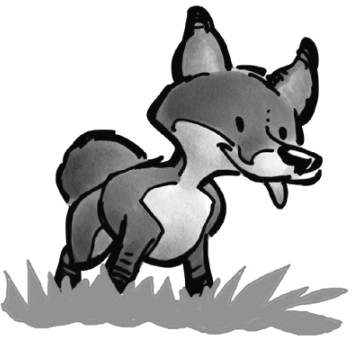
\includegraphics[width=\textwidth]{fox.png}
\end{minipage}
\end{lyrics}
\end{figure}
\vspace{-15pt}
\begin{center}
    \songtitle{$\delta6$e}{Supen} 
    \mel{Räven}
\end{center}
\vspace{-10pt}
\begin{lyrics}
Jag fångade en sup idag \\
men supen slank ur näven, \\
men lika gla' för det är ja' \\
men gladast är nog levern! 
\vspace{5pt} \\
Lala lalalala...
\vspace{5pt} \\
Jag fångade en PRezt idag \\
men prästen damp i gatan, \\
men lika gla' för det är ja' \\
men gladast är nog Satan!
\vspace{5pt} \\
Lala lalalala...
\vspace{5pt} \\
Jag fångade en biff idag \\
men den var seg som kola \\
och lika seg som den är ja'. \\
Det är så kul att skåla! 
\end{lyrics}

\nysida{4}{7}
\noindent
\begin{center}
    \songtitle{$\delta7$a}{Nu ska vi klämma septen} 
    \mel{Nu ska vi skörda linet}
\end{center}
\begin{lyrics}
Nu skall vi klämma septen gutår, \\
sjunga en trudelutt om det går. \\
Tjosan Muhammed, nu är det vår, \\
julafton är en fredag. 
\vspace{5pt} \\
Klunk-klunk-klunk, klunk-klunk-klunk, \\
blanda och ge, blanda och ge, \\
abra kadabra klunk, \\
julafton är en fredag. \\\digitalonly{\\}
\textit{(om och om igen, fortare och fortare)}
\end{lyrics}
\begin{center}
    \songtitle{$\delta7$b}{Full och galen} 
    \mel{Kors på Idas grav (Imbelupet)}
\end{center}
\begin{lyrics}
Full och galen med moralen minimal, \\
ljuder nu signalen till vår bacchanal. \\
Sensmoralen i lokalen \\
är att tömma sin pokal \\
så skandalen i finalen blir total.
\end{lyrics}
\begin{center}
    \songtitle{$\delta7$c}{Toj hemtegubbar} 
    \mel{Hej tomtegubbar}
\end{center}
\begin{lyrics}
$\|$: Toj hemtegubbar gla i slåsen \\
och låt oss vastiga lura! :$\|$
\vspace{5pt} \\
En liten tid vi heva lär \\
Med möcken hyda och svär bestor, \\
Toj hemtegubbar gla i slåsen \\
och låt oss vastiga lura.
\end{lyrics}

\newpage
\noindent
\begin{center}
    \songtitle{$\delta7$d}{Full är bäst} 
    \mel{Vi gå över daggstänkta berg}
\end{center}
\begin{lyrics}
Vi som oss för att glupa satt \\
supa glatt, \\
ity den som försmår sin första tår \\
törsta får. \\
Av längtan vi tryckas, av trängtan att lyckas, \\
vi nu med bravur häller ur, \\
eller hur? 
\vspace{5pt} \\
Vi ger tätt som titt strupen sitt, \\
supen stritt \\
skall forsa och snart får sig tarmen vår \\
varm en tår. \\
Er öven i seder, och söven sen ned er\\ 
på denna protestbullerfest, \\
full är bäst! 
\end{lyrics}
\begin{center}
    \songtitle{$\delta7$e}{Morsgrisar små} 
    \mel{Morsgrisar är vi allihopa}
\end{center}
\begin{lyrics}
Morsgrisar små ska inte supa \\
för de stupa allihopa. \\
Men vi vill ha brännvin fyllt med skupa \\
i våra djupa strupa. 
\vspace{5pt} \\
Nu med, \textit{(supen tas) }\\
och nu med. \textit{(tupen sas) }\\
Nu med, \textit{(schupen tasch) }\\
och nu med. \textit{(schnaps) }
\end{lyrics}

\nysida{4}{8}
\noindent
\begin{center}
    \songtitle{$\delta8$a}{Livet är härligt} 
    \mel{Polyushko-polye}
    \instruction{Sjunges först svagt, sedan starkt}
\end{center}
\begin{lyrics}
$\|$: Livet är härligt!\\
Tavaritj, vårt liv är härligt!\\
Vi alla våra små bekymmer glömmer\\
när vi har fått en tår på tanden, skål!\\
Tag dig en vodka!\\
Tavaritj, en liten vodka!\\
Glasen i botten vi tillsammans tömmer! 
\vspace{5pt}\\
1: Det kommer mera efter ha-a-and. :$\|$
\vspace{5pt}\\
2: Det kommer mera efter hand! 
\end{lyrics}
\auth{Chalmersspexet Katarina 1959\\Denna sjunges först på alla Chalmerssittningar}
\begin{center}
    \songtitle{$\delta8$b}{Vodka, vodka} 
    \mel{Stenka Razin}
\end{center}
\begin{lyrics}
Vodka, vodka vill jag dricka, \\
jag vill äta kaviar, \\
$\|$: jag vill älska russkij männ'ska, \\
jag vill spy i samovar :$\|$
\vspace{5pt}\\
Vita möss som gå i taket, \\
råma hest och falla ned, \\
$\|$: men ni skall inte var rädda, \\
ta en sup och allt går väl :$\|$
\vspace{5pt}\\
Uppå väggen går en gädda, \\
med långa ludna, svarta ben, \\
$\|$: men ni skall inte var rädda, \\
ta en sup och allt går väl :$\|$
\digitalonly{
\\\\\\(Varianter på första versen)
Falu brännvin - falukorv - falu människa - Faluån
Whisky - baked beans - Yankee människa - på mina jeans
En kan också permutera "äta", "älska" och "spy i"
}
\end{lyrics}

\newpage
\noindent
% TODO: Digitalize
\textit{Varianter på första versen:}
\vspace{5pt}\\
Falu brännvin - falukorv - falu - Faluån
\vspace{5pt}\\
Whisky - baked beans - Yankee - på mina jeans
\vspace{5pt}\\
En kan också permutera "äta", "älska" och "spy i".
\vspace{10pt}
\begin{center}
    \songtitle{$\delta8$c}{Så hastigt} 
    \mel{Flickan går i ringen}
\end{center}
\begin{lyrics}
Så hastigt den lilla nubben i strupen försvann, \\
Så hastigt den lilla nubben i strupen försvann. \\
Håhå jaja, kommer rafflan idag, \\
Håhå jaja, kommer rafflan idag? 
\end{lyrics}
\vspace{10pt}
\begin{center}
    \songtitle{$\delta8$d}{Gräv ur tundran} 
    \mel{Katyuscha}
\end{center}
\begin{lyrics}
Gräv ur tundran två dussin potäter \\
låt dem jäsa uti fjorton dar. \\
$\|$: Modersmjölken för ryssar och sovjeter, \\
brännes i babusjkans samovar :$\|$
\vspace{5pt}\\
Kyl sen drycken i Sibiriens tjäle, \\
tappa upp på immiga små glas. \\
Höj sen glasen för fosterlandets välgång, \\
sjung "Nastrovie" med en mäktig bas. \\
Höj sen glasen för fosterlandets välgång, \\
sjung "Nastrovie"... \textit{(supen intages)} \\
låt glasen gå i kras! 
\end{lyrics}
\auth{Ekonomspexet Lenin 1989}

\nysida{4}{9}
\noindent
\begin{center}
    \songtitle{$\delta9$a}{Hyllning till OP Andersson} 
    \mel{Lilie Marlene (Gul lyser solen)}
    \instruction{(Inte "Vi äro musikanter")}
\end{center}
\begin{lyrics}
Vi kan dricka Sädes \\
och vi kan dricka Kron. \\
Men allra mest vi glädes, \\
åt OP Andersson.
\vspace{5pt}\\
När den gått ned uti vår strup, \\
så ropas det på nästa sup: \\
ur svenska hjärtans djup, \\
ur svenska hjärtans djup. 
\end{lyrics}
\vspace{30pt}
\begin{center}
    \songtitle{$\delta9$b}{Tänk om jag hade lilla nubben...} 
    \mel{Hej tomtegubbar}
\end{center}
\begin{lyrics}
$\|$: Tänk om jag hade lilla nubben \\
uppå ett snöre i halsen! :$\|$
\vspace{5pt}\\
Och kunde dra den upp och ner \\
så att den smaka' som många fler! \\
Tänk om jag hade lilla nubben \\
uppå ett snöre i halsen 
\end{lyrics}

\newpage
\noindent
\begin{center}
    \songtitle{$\delta9$c}{Krök armen} 
    \mel{Väva vadmal}
\end{center}
\begin{lyrics}
Krök armen i vinken, \\
här vankas det finkel. \\
Och vanka finkel \\
och finka vankel \\
och kröka armen i finkel. \\
Här vankas det vinkel. 
\end{lyrics}
\begin{center}
    \vspace{40pt}
    \songtitle{$\delta9$d}{Inre dialog} 
    \mel{An der schönen blauen Donau}
    \instruction{\physicalonly{Försångare/\textbf{Alla}}\digitalonly{F: Försångare\\A: Alla}}
\end{center}
\begin{lyrics}
\forsangare{Jag vill inte ha} - \alla{en nubbe till!}\\
\forsangare{Jag mår inte bra} - \alla{en nubbe till!}\\
\forsangare{Om ni ger mig mer} - \alla{en nubbe till!}\\
\forsangare{ser jag er som fler} - \alla{en nubbe till!}\\
\vspace{5pt}
\forsangare{Min mage är sjuk} - \alla{en nubbe till!}\\
\forsangare{Min hjärna är mjuk} - \alla{en nubbe till!}\\
\forsangare{Jag kan inte tänka så bra,\\
så jag får väl nubben ta - hurra!}\\
\end{lyrics}
\auth{Mikael Segersten (E\digitalonly{-76})}

\nysida{4}{10}
\noindent
\begin{center}
    \songtitle{$\delta10$a}{Månvisa} 
\end{center}
\begin{lyrics}
När månen vandrar sin tysta ban \\
och tittar in genom rutan \\
Då tänker jag att på ljusa dan \\
då kan jag klara mig utan. \\
Ja, jag kan klara mig utan måne, \\
men utan renat och utan Skåne, \\
det vete f-n, det vete f-n. 
\end{lyrics}
\begin{center}
    \songtitle{$\delta10$b}{Måsen}
    \mel{Månvisa} 
\end{center}
\begin{lyrics}
Det satt en mås på en klyvarbom, \\
och torr i krävan var kräket. \\
Och torkan brände i skepparns gom, \\
när de låg där i bleket. \\
"Jag vill ha sill" hördes måsen rope, \\
Och skepparn svarte "Jag vill ha OP \\
om blott jag får, om blott jag får" 
\vspace{5pt}\\
Nu lyfte måsen från klyvarbom \\
och vinden spelar i tågen \\
och OP:n svalkade skepparns gom. \\
Jag önskar blott att jag såg 'en. \\
Så arm och nykter den arme kraken \\
hen sätter storsegel den krabaten. \\
Till sjöss hen far och halvan tar. 
\end{lyrics}

\begin{center}
    \songtitle{$\delta10$c}{Den vingklippta måsen} 
\end{center}
\begin{lyrics}
Det satt en mås på en klyvarbom\\
Jag vill ha OP! 
\end{lyrics}

\newpage
\noindent
\begin{center}
    \songtitle{$\delta10$d}{JASen} 
    \mel{Månvisa}
\end{center}
\begin{lyrics}
Det flög en JAS över Västerbron \\
men styrsystemet var trasigt. \\
Piloten sköt ut sig med kanon \\
för planet svängde så knasigt. \\
"Jag vill ju uppåt, jag vill ju mer"\\
men planet svarte: "Jag vill ju ner"\\
mot alla hjon på Västerbron. 
\end{lyrics}
\auth{Dadderiet 1993}

\begin{center}
    \songtitle{$\delta10$e}{När nubben blänker} 
    \mel{Månvisa}
\end{center}
\begin{lyrics}
När nubben blänker i immigt glas \\
som hoppets strålande stjärna, \\
då är det avsett att det ska tas \\
förutan fruktan och gärna. \\
Så klang och klingom, så tar vi supen, \\
den läskar härligt den torra strupen. \\
Ja, skål gutår, ja, skål gutår! 
\end{lyrics}

\begin{center}
    \songtitle{$\delta10$f}{Moose:en} 
    \mel{Månvisa}
\end{center}
\begin{lyrics}
Det satt en älg i en klyvartopp,\\
förklädd i älgjaktens månad.\\
Befjädrad var hen från tå till topp,\\
skepparn blev rätt förvånad.\\
"Jag är en mås, goa skepparn!", ljög den\\
förklädda älgen, därefter flög den.\\
Mjukt föll den sen, på skepparen.
\end{lyrics}

\newpage
\noindent
\begin{center}
    \songtitle{$\delta10$g}{När jag är fuller} 
    \mel{Månvisa}
\end{center}
\begin{lyrics}
När jag är fuller, då är jag glad, \\
fan vet om jag ej är vacker. \\
Då går jag runt i vår lilla stad, \\
ibland lyxhus och baracker. \\
Jag sjunger stilla en serenad, \\
det gör jag bara när jag är glad, \\
och full och vacker, och full och vacker. 
\vspace{5pt}\\
När jag är fuller då är jag stark, \\
fan vet om jag ej är modig. \\
Då kan jag slå vem som helst i mark, \\
så hen blir trasig och blodig. \\
Jag välter träden uti vår park, \\
det gör jag bara när jag är stark, \\
och full och modig, och full och modig. 
\vspace{5pt}\\
När jag är fuller då är jag rik, \\
fan vet om jag ej är snille. \\
Och dör jag blir jag ett vackert lik, \\
begravd med gravöl och gille. \\
I himlen möts jag av hornmusik, \\
det gör en bara när en är rik, \\
och är ett snille, och är ett snille.
\vspace{5pt}\\
Men om jag kvicknar till ett litet slag, \\
i något enkelrum med galler. \\
Då känner jag mig så rysligt svag, \\
och avskyr bråk och kravaller. \\
Min mage krånglar och är ur lag, \\
och fan ska veta att jag idag \\
är bakom galler, är bakom galler. 
\end{lyrics}
\auth{Sångartäflan 1942}

\newpage
\noindent
\begin{center}
    \songtitle{$\delta10$h}{Mesen} 
    \mel{Månvisa}
\end{center}
\begin{lyrics}
Det satt en mes i en klyvarmast,\\
där sågs hen ragla och svaja.\\
För trots att frön var hens enda last,\\
var hen nu full som en kaja.\\
"Vad har du gjort!" hördes skepparn stöna\\
och mesen svarte: "Jag rökte fröna!\\
I egen holk, i egen holk"
\end{lyrics}
\begin{center}
    \songtitle{$\delta10$i}{Musen} 
    \mel{Månvisa}
\end{center}
\begin{lyrics}
Det satt en mus i en hushållsost,\\
och åt och åt utan måtta.\\
Tills osten blivit en mushåls-ost,\\
och hen en klotformad råtta.\\
"Så bra", sa musen, "att va en fettboll,\\
nu kan jag rulla med hast åt rätt håll:\\
Ostindien! Ostindien!"
\end{lyrics}
\begin{center}
    \songtitle{$\delta10$j}{Måsens sista sup} 
    \mel{Månvisa}
\end{center}
\begin{lyrics}
Den mås som satt på en klyvarbom,\\
den är nu död och begraven\\
Och skepparn som drack en flaska rom,\\
hen har nu drunknat i haven.\\
Så kan det gå om en fått för mycke'\\
om en för brännvin har fattat tycke.\\
Vi som har kvar, vi resten tar.
\end{lyrics}

\nysida{4}{11}
\noindent
\begin{center}
    \songtitle{$\delta11$a}{Humlorna} 
    \mel{Karl Alfred boy}
\end{center}
\begin{lyrics}
Vi äro små humlor vi, bzzz, bzzz. \\
Vi äro små humlor vi, bzzz, bzzz. \\
Vi äro små humlor som tar oss en geting. \\
Vi äro små humlor vi, bzzz, bzzz. 
\end{lyrics}
\begin{center}
    \songtitle{$\delta11$b}{Fiskarna} 
    \mel{Karl Alfred boy}
\end{center}
\begin{lyrics}
Vi äro små fiskar vi, blubb, blubb. \\
Vi äro små fiskar vi, blubb, blubb. \\
Vi äro små fiskar som tar oss en kallsup. \\
Vi äro små fiskar vi, blubb blubb. 
\end{lyrics}
\begin{center}
    \songtitle{$\delta11$c}{Änglarna} 
    \mel{Karl Alfred boy}
\end{center}
\begin{lyrics}
Vi äro små änglar vi, flax, flax.\\
Vi äro små änglar vi, flax, flax.\\
Vi äro små änglar som tar oss en djävel.\\
Vi äro små änglar vi, flax, flax.
\end{lyrics}
\begin{center}
    \songtitle{$\delta11$d}{Brännvin är jävligt gott}
    \mel{Karl Alfred boy}
\end{center}
\begin{lyrics}
Ja, brännvin är jävligt gott. \textit{(bank, bank)}\\
Blir bättre ju mer en fått. \textit{(bank, bank)}\\
Det rinner längs halsen, en tappar balansen. \\
Ja, brännvin är jävligt gott! \textit{(bank, bank)}
\newpage
\noindent
Ja, brännvin är jävligt gott. \textit{(bank, bank)}\\
Blir bättre ju mer en fått. \textit{(bank, bank)}\\
Men går en i golvet, så där framåt tolv-ett. \\
Så slår en sig jävligt hårt! \textit{(bank, bank)}
\end{lyrics}
\vspace{20pt}
\begin{center}
    \songtitle{$\delta11$e}{En liten fyllhund}
    \mel{Mors lilla Olle}
\end{center}
\begin{lyrics}
En liten fyllhund på krogen satt. \\
Rosor på kinden - men blicken var matt. \\
Läpparna små liksom näsan var blå. \\
Bara jag kunde så skulle jag gå. 
\end{lyrics}
\vspace{20pt}
\begin{center}
    \songtitle{$\delta11$f}{Getingen}
    \mel{Jazzgossen}
\end{center}
\begin{lyrics}
Å så kommer det en geting, \\
genom luften som ett reaplan. \\
Å hen åker på en snyting, \\
mitt under röda kran. \\
Å hen trillar ner i magen, \\
med ett jätteplask, \\
jätteplask, jätteplask. \\
Å så blir en lite dragen, \\
men pigg och rask, \\
pigg och rask, pigg och rask. 
\end{lyrics}

\newpage
\noindent
\begin{center}
    \songtitle{$\delta11$g}{Kalla små nubbar} 
    \mel{Kalle på spången}
    \instruction{\physicalonly{Försångare/\textbf{Alla}}\digitalonly{F: Försångare\\A: Alla}}
\end{center}
\begin{lyrics}
\forsangare{Vad är det som gör \\
att en skojare trivs?} \\
\alla{Jo, kalla, kalla, kalla, kalla \\
små nubbar. \\}
\forsangare{Vad är det som först \\
uppå festen väl givs?} \\
\alla{Jo, kalla, kalla, kalla, kalla \\
små nubbar. \\}
\forsangare{Dom skänker oss alla \\
ett solljust humör, \\
och även för kroppen \\
stor nytta dom gör. \\
Men skall en ta nubbar \\
så regel dom bör \\
va' kalla.} \\
\alla{Mycket kalla.\\}
Ja, kalla. \\
\alla{Mycket kalla.\\
Ja, kalla, kalla, kalla, kalla \\
små nubbar. }
\end{lyrics}

\nysida{4}{12}
\noindent
\begin{center}
    \songtitle{$\delta12$a}{Mod i barm} 
    \mel{Kungssången}
\end{center}
\begin{lyrics}
Ur svenska hjärtans djup en sup, \\
en samfälld och en enkel sup \\
som ger oss mod i barm. \\
I prima äktsvensk alkohol \\
för svenska folkets höga mål \\
vi höjer nu vår första skål, \\
vi ungdoms främsta vän.
\end{lyrics}
\begin{center}
    \songtitle{$\delta12$b}{Oh Besinna} 
    \mel{Oh, Susanna}
\end{center}
\begin{lyrics}
Smuttans ungar har just runnit ner \\
uti magens boudoir. \\
Kommer inte genast något mer, \\
Höres magens kommentar. \\
Oh besinna, den saken är ju klar, \\
både tarmvred, magsår och kolik \\
dunstar bort med lite sprit. 
\end{lyrics}
\begin{center}
    \songtitle{$\delta12$c}{Mera järn} 
    \mel{Milord}
\end{center}
\begin{lyrics}
Vi vill ha mera järn, \\
vi vill ha flera järn, \\
ett litet rostfritt, oböjt, \\
destillerat järn! \\
Och vi ska böja järn, \\
och vi ska kröka järn \\
så att vi har det \\
flytande i morgon kväll.
\end{lyrics}

\newpage
\noindent
\begin{center}
    \songtitle{$\delta12$d}{Vem kan kröka} 
    \mel{Vem kan segla}
\end{center}
\begin{lyrics}
Vem kan kröka förutan krök? \\
Vem kan gå utan vingel? \\
Vem kan skala en stor gul lök, \\
utan att fälla tårar? 
\end{lyrics}
\vspace{40pt}
\begin{center}
    \songtitle{$\delta12$e}{Vem kan hugga} 
    \mel{Vem kan segla}
\end{center}
\begin{lyrics}
Vem kan hugga sig själv i knät? \\
Vem kan slå sig på tummen? \\
Vem kan skära i vännen sin, \\
utan att dra på munnen? 
\vspace{5pt}\\
Jag kan hugga mig själv i knät,\\
Jag kan slå mig på tummen, \\
Men ej skära i vännen min, \\
utan att dra på munnen. 
\vspace{5pt}\\
Vem kan ragla förutan vin? \\
Vem är nykter om våren? \\
Vem kan skilja på kron och gin, \\
utan att smaka på'ren? 
\vspace{5pt}\\
Jag kan ragla förutan vin, \\
Och visst var jag nykter om våren, \\
men ej skilja på kron och gin, \\
efter den elfte tåren.
\end{lyrics}

\nysida{4}{13}
\noindent
\begin{center}
    \songtitle{$\delta13$a}{Var redo!} 
    \mel{Ur vägen}
\end{center}
\begin{lyrics}
$\|$: Var redo, var redo, \\
För nu skall supen tas :$\|$\\
Den gör gott åt kroppen och åt själen, \\
känns ifrån hjässan långt ned i hälen. \\
Kling, klang, kling, klang, \\
nu börjar vårt kalas. 
\end{lyrics}
\digitalonly{\auth{C.M. Bellman}}
\vspace{20pt}
\begin{center}
    \songtitle{$\delta13$b}{Till supen så tager en sill} 
    \mel{Daggstänkta berg}
\end{center}
\begin{lyrics}
Till supen så tager en sill, sill, sill, \\
men också ansjovis om en vill, vill, vill. \\
$\|$: Och om en är oviss om sillen är ansjovis, \\
så tar en bara några supar till, till, till. :$\|$
\end{lyrics}
\vspace{20pt}
\begin{center}
    \songtitle{$\delta13$c}{Vi går över ån} 
    \mel{Daggstänkta berg}
\end{center}
\begin{lyrics}
Vi går över ån efter sprit, fallera!\\
Men efter vatten går vi ej en bit, fallera!\\
Ja sup kära vänner\\
fast näsan den ränner,\\
en gång så blir den ack va vit, fallera!
\end{lyrics}

\newpage
\noindent
\begin{center}
    \songtitle{$\delta13$d}{Sänkta Lucia} 
    \mel{Sankta Lucia}
\end{center}
\begin{lyrics}
Huvet slåt kopparslag, ögonen svider,\\
i magen obehag, natten den lider.\\
Då genom strupen går\\
hembränt en liten tår.\\
Vördat vare vårat brännvin,\\
vördat vårt brännvin.
\end{lyrics}
\vspace{40pt}
\begin{center}
    \songtitle{$\delta13$e}{Lundströms kök} 
    \mel{Ska det verkligen behövas någon melodi?}
\end{center}
\begin{lyrics}
Trrrrrretton kärringar i Lundströms kök, \\
i Lundströms kök, i Lundströms kök. \\
Alla var de fulla utom en som söp, \\
en som söp sig full, skål! 
\end{lyrics}

\nysida{4}{14}
\noindent
\begin{center}
    \songtitle{$\delta14$a}{Solen} 
    \mel{Camptown Ladies}
\end{center}
\begin{lyrics}
Solen den går upp och ner, doda, doda! \\
Jag ska aldrig supa mer, hej doda dej! \\
Hej doda dej, hej doda dej! \\
Jag ska aldrig supa mer, hej doda dej! 
\vspace{5pt} \\
Men detta var ju inte sant, doda, doda! \\
I morgon gör jag likadant, hej doda dej! 
\end{lyrics}
\vspace{10pt}
\begin{center}
    \songtitle{$\delta14$b}{Korta solen} 
\end{center}
\begin{lyrics}
Solen den går upp och ner, snapsen den går ner!
\end{lyrics}
\vspace{25pt}
\begin{center}
    \songtitle{$\delta14$c}{Old Janx Spirit} 
    \mel{When Johnny Comes Marching Home}
\end{center}
\begin{lyrics}
Oh don't give me none more of that \\
Old Janx Spirit! \\
No, don't you give me none more of that \\
Old Janx Spirit! \\
For my head will fly, \\
my tongue will lie \\
my eyes will fry \\
and I may die. \\
Won't you pour me one more \\
of that sinful Old Janx Spirit. 
\end{lyrics}
\auth{Gruvarbetarsång från Orion}

\nysida{4}{15}
\noindent
\begin{center}
    \songtitle{$\delta14$e}{Hörapparaten} 
    \mel{Jenka}
\end{center}
\begin{lyrics}
Brännvin, öl, och gammal finkel \\
gör att jag jag nu ser i vinkel. \\
Därför hamnar inte supen (alt. maten) \\
uti strupen utan i min hörapparat.\\
\end{lyrics}

\begin{center}
    \songtitle{$\delta15$a}{Göken} 
    \mel{Räven raskar över isen}
\end{center}
% TODO: Digitalize Lyrics 
\vspace{-10pt}
\begin{lyrics}
\begin{table}[!h]
\begin{tabularx}{0.85\textwidth}{l l}
\physicalonly{\textbf{\small Osquar:}}\digitalonly{Ett bord:} &\small Och nubben kallas också göken. \\
 &\small Och nubben kallas också göken. \\
 &\small Säg, får jag lov, säg, får jag lov, \\
 &\small att byta byxor i kröken? \\
&\\
\physicalonly{\textbf{\small Osqulda:}}\digitalonly{Ett annat bord:} &\small Nej, det går inte alls, mitt herrskap, \\ 
 &\small det går inte alls, mitt herrskap. \\
 &\small För se ni har, för se ni har \\
 &\small ju inga byxor dessvärre. 
\end{tabularx}
\end{table}
\end{lyrics}
\begin{center}
    \songtitle{$\delta15$b}{Magen brummar} 
    \mel{Broder Jakob\digitalonly{\\Kanon}}
    \textit{Kanon} % Not parsed by JSON parser
\end{center}
\begin{lyrics}
Magen brummar. \\
Jag försummar \\
hälla dit \\
mera sprit. \\
Nu så ska vi dricka, \\
så att vi får hicka. \\
Mera sprit. \\
Akvavit. 
\end{lyrics}

\newpage
\noindent
\begin{center}
    \songtitle{$\delta15$c}{Gammalt brännvin} 
    \mel{Gubben Noak}
\end{center}
\begin{lyrics}
Gammalt brännvin, \\
gammalt brännvin \\
finnes i vårt krus. \\
Vänner slå i glasen, \\
mången stora snapsen \\
Gån till verket, \\
gån till verket! \\
Tag ett stadigt rus! 
\vspace{5pt}\\
Gammalt brännvin, \\
gammalt brännvin \\
flödar i vår kropp. \\
Genom torra strupar \\
rinna starka supar. \\
Ge åt kroppen, \\
ge åt själen \\
kraft och frejdigt hopp! 
\end{lyrics}
\vspace{50pt}
\begin{center}
    \songtitle{$\delta15$d}{Månen (En gång i månan)}
    \mel{Mors lilla Olle}
\end{center}
\begin{lyrics}
En gång i månan är månen full, \\
men aldrig jag sett henom ramla omkull. \\
Stum av beundran hur mycket hen tål, \\
höja vi glasen och dricka hens skål. 
\end{lyrics}

\nysida{4}{16}
\noindent
\begin{center}
    \songtitle{$\delta16$a}{Raj-Raj} 
    \mel{Kväsarvalsen}
\end{center}
\begin{lyrics}
Ingen har det så bra som jag, \\
nej, ingen har det så bra som jag, \\
förutom min vän som, så vitt jag vet, \\
ligger i sprit uppå Riksmuseet. 
\vspace{5pt}\\
Raj-raj-raj... 
\end{lyrics}
\vspace{20pt}
\begin{center}
    \songtitle{$\delta16$b}{Tjugotre} 
    \mel{Amanda Lundbom}
\end{center}
\begin{lyrics}
Tjugotre är Bäska Droppar, \\
bom-faderia, bomfaderaderalla. \\
skänker liv åt döda kroppar, \\
bom-faderi, faderallanlej. 
\vspace{5pt}\\
Slå en sup i död väns kropp, \\
bom-faderi, faderallanlej. Hugg i! \\
så stapplar hen ur graven opp, \\
bom-faderi faderallanlej. 
\vspace{5pt}\\
Jesus visste att de döda, \\
bom-faderia, bomfaderaderalla, \\
kunde väckas utan möda, \\
bom-faderi faderallanlej. 
\vspace{5pt}\\
Bäska Droppar nyttja' han, \\
Bom-faderi, faderallanlej, Hugg i! \\
och Lazarus spratt till, minsann, \\
bom-faderi faderallanlej. 
\end{lyrics}
\auth{Carl Nisser, E-80}

\newpage
\noindent
\begin{center}
    \songtitle{$\delta16$c}{Vikingen} 
    \mel{When Johnny Comes Marching Home}
\end{center}
\begin{lyrics}
En viking älskar livets vand, \\
hurra, hurra! \\
Det hastigt i hens svalg försvann, \\
hurra, hurra! \\
Till kalv, till oxe, till fisk, till fläsk, \\
när alla veklingar dricker läsk. \\
Ja, då vill alla vikingar ha en bäsk. 
\vspace{5pt}\\
När bäsken småningom är slut, \\
tragik, tragik. \\
Då bärs varenda viking ut \\
som lik, sig lik. \\
Och sen när vi vaknar, vi sjunger en bit, \\
och korkar upp skånes akvavit. \\
Skål för alla vikingar som kom hit. 
\end{lyrics}
\auth{Sångarstriden 1981}
\newpage\begin{center}
    \songtitle{$\delta16$d}{Feministvikingen} 
    \mel{When Johnny Comes Marching Home}
\end{center}
\begin{lyrics}
En viking viker tvätten själv,\\
hurra, hurra!\\ 
Ordet viking härstammar\\ 
därav, jaha!\\ 
Föräldraledighet delas exakt, \\
Och när herr viking barnen lagt,\\ 
Då är vikingens fru ute på jakt! 
\vspace{5pt}\\
En viking älskar livets vann,\\
hurra, hurra! \\
Men på sig själv han lägger band,\\
vad bra, vad bra! \\
Mjödet prioriteras sist,\\
Kök och städ blir aldrig trist,\\ 
För vår viking han är feminist! 
\end{lyrics}

\auth{Hittad av Linn Odelius, F-15}
\nysida{4}{17}
\noindent
\begin{center}
    \songtitle{$\delta17$a}{Uti min mage} 
    \mel{Uti vår hage}
\end{center}
\begin{lyrics}
Uti min mage en längtan mig tär. \\
Kom hjärtans fröjd. \\
Där råder en hunger som ropar så här: \\
Kom kryddsill och kall potatis. \\
Kom brännvin och quantum satis. \\
Kom allt som kan drickas, kom hjärtans fröjd. 
\vspace{5pt}\\
Uti mitt hjärta en längtan mig tär. \\
Kom hjärtans fröjd. \\
Där råder en hunger som ropar så här: \\
Kom famnande lena armar. \\
Kom läppar och sköna barmar. \\
Kom fagraste människor. \\
Kom hjärtans fröjd. 
\vspace{5pt}\\
Uti vår mage där växa begär. \\
Kom hjärtans kär. \\
Vill du mig något så träffas vi där. \\
Kom Renat och Aqua Vitae. \\
Kom OP och allt vad sprit e'. \\
Kom ljuva Genever. \\
Kom Överste. 
\end{lyrics}

\newpage
\noindent
\begin{center}
    \songtitle{$\delta17$b}{Då verka lätt} 
    \mel{Dover Calais}
\end{center}
\begin{lyrics}
När jag tar mig en sup \\
blir jag intressant och djup. \\
Allting som är svårt \\
kan då verka lätt. 
\vspace{5pt}\\
All min rädsla går bort \\
med en grogg av någon sort. \\
Allting som är svårt \\
kan då verka lätt! 
\end{lyrics}

\end{document}